\part{}
\chapter{Eccentric Connections}
\section{Types of Connections}
Some of the principles of bolted steel connections are similar. We will treat them together in this section.
\begin{figure}[H]
\begin{tikzpicture}
\node at(0,0){\includegraphics[height=6cm]{PIC/CH06/BBP2}};
\draw[->,line width=2mm,cc0066](1,1)--++(-90:2);
\end{tikzpicture}\hfil
\begin{tikzpicture}
\node at(0,0){\includegraphics[height=6cm]{PIC/CH06/BBP}};
\draw[->,line width=2mm,cc0066](2,2)--++(-90:2);
\end{tikzpicture}\hfil
\begin{tikzpicture}
\node at(0,0){\includegraphics[height=6cm]{PIC/CH08/ECC}};
\draw[->,line width=1.4mm,cc0066](.5,1.5)--++(-90:1.5);
\draw[->,line width=1.4mm,cc0066](-1.5,-1)--++(-90:1.5);
\end{tikzpicture}
\end{figure}
\section{Eccentric Bolted Connections}
Bolts are subject to different shear forces, two design methods exist, namely,
\begin{itemize}
\item Elastic Design Method --- simple, slightly conservative
\item Ultimate Strength Method --- manuals
\end{itemize}
\subsection{Elastic Design Method}
%The external load $P$ is decomposed into two components: direct shear and torsion. It is equivalent to shifting $P$ to the centre of rigidity (c.r.).
\begin{figure}[H]
\centering\footnotesize
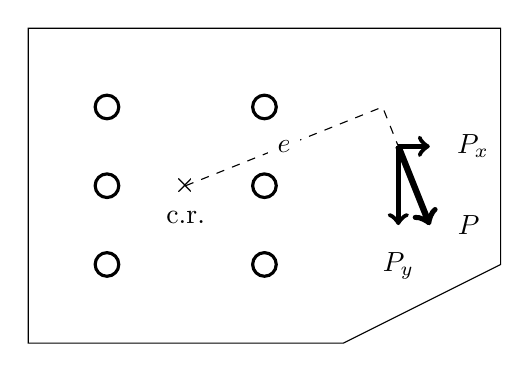
\begin{tikzpicture}
\draw(-1,-1)--++(4,0)--++(2,1)--++(0,3)-|cycle;
\foreach\x in{0,2}{
\foreach\y in{0,1,2}{
\node[circle,inner sep=0pt,minimum size=3mm,line width=.4mm,draw]at(\x,\y){};}}
\draw(1,1)node{\texttimes}node[below=2mm]{c.r.};
\draw[dashed](1,1)--++(2.5,1)node[fill=white,midway]{$e$}--++(.2,-.5)coordinate(A);
\draw[->,line width=.8mm](A)--++(.4,-1)node[right=2mm]{$P$};
\draw[->,line width=.6mm](A)--++(.4,0)node[right=2mm]{$P_x$};
\draw[->,line width=.6mm](A)--++(0,-1)node[below=2mm]{$P_y$};
\end{tikzpicture}\caption{Decomposition of arbitrary force into $x$ and $y$ components}
\end{figure}
\subsubsection{Basis for Elastic Computation}
\paragraph{Assumption}
Basic assumptions for elastic computations are made as follows.
\begin{itemize}
\item Connector plate is rigid.
\item Fasteners deform elastically.
\item Fastener forces can be split into direct shear and torsional shear forces with appropriate vectorial components.
\end{itemize}
\paragraph{Notation}
The following notations will be used in the analysis.
\begin{conditions}
B_i&fastener direct shear force\\
B_{i,x}&fastener direct shear force component in $x$ direction\\
B_{i,y}&fastener direct shear force component in $y$ direction\\
P&applied force\\
P_x&applied force component in $x$ direction\\
P_y&applied force component in $y$ direction\\
r_i&(positive) distance from c.r. (centre of rigidity) to fastener $i$\\
k_i&fastener stiffness\\
e&eccentricity\\
\theta&plate rotation\\
\delta_i&fastener deformation due to plate rotation $\theta$\\
x_{cr}&$x$ coordinate of c.r. in the appropriate coordinate system\\
y_{cr}&$y$ coordinate of c.r. in the appropriate coordinate system\\
T_i&fastener force due to applied torque
\end{conditions}
\paragraph{Equilibrium} In-plane forces shall satisfy statics equilibrium equations.
\begin{align}
\sum{}F_x=0,\quad&\longrightarrow\quad\sum_{i=1}^nB_{i,x}=P_x,\\
\sum{}F_y=0,\quad&\longrightarrow\quad\sum_{i=1}^nB_{i,y}=P_y,\\
\sum{}M=0,\quad&\longrightarrow\quad\sum_{i=1}^nT_ir_i=Pe.
\end{align}
\begin{figure}[H]
\centering\scriptsize
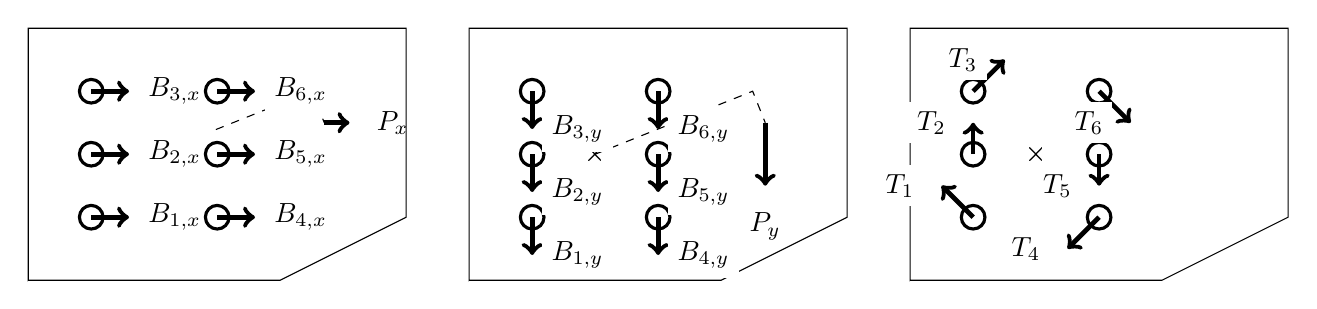
\begin{tikzpicture}[scale=.8]
\draw(-1,-1)--++(4,0)--++(2,1)--++(0,3)-|cycle;
\draw(1,1)node{\texttimes};
\draw[dashed](1,1)--++(2.5,1)--++(.2,-.5)coordinate(A);
\draw[->,line width=.6mm](A)--++(.4,0)node[right=2mm]{$P_x$};
\foreach\x in{0,2}{\foreach\y[evaluate=\y as \z using int(1+\y+1.5*\x)]in{0,1,2}{
\node[circle,inner sep=0pt,minimum size=3mm,line width=.4mm,draw]at(\x,\y){};
\draw[->,line width=.6mm](\x,\y)--++(.6,0)node[right=1mm,fill=white]{$B_{\z,x}$};}}
\begin{scope}[xshift=7cm]
\draw(-1,-1)--++(4,0)--++(2,1)--++(0,3)-|cycle;
\draw(1,1)node{\texttimes};
\draw[dashed](1,1)--++(2.5,1)--++(.2,-.5)coordinate(A);
\draw[->,line width=.6mm](A)--++(0,-1)node[below=2mm]{$P_y$};
\foreach\x in{0,2}{\foreach\y[evaluate=\y as \z using int(1+\y+1.5*\x)]in{0,1,2}{
\node[circle,inner sep=0pt,minimum size=3mm,line width=.4mm,draw]at(\x,\y){};
\draw[->,line width=.6mm](\x,\y)--++(0,-.6)node[right=1mm,fill=white]{$B_{\z,y}$};}}
\end{scope}
\begin{scope}[xshift=14cm]
\draw(-1,-1)--++(4,0)--++(2,1)--++(0,3)-|cycle;
\draw(1,1)node{\texttimes};
\setstructmech{convention=direction}
\NodalForce{1,1}[N][N][-Pe]
\foreach\x in{0,2}{\foreach\y[evaluate=\y as \z using int(1+\y+1.5*\x)]in{0,1,2}{\node[circle,inner sep=0pt,minimum size=3mm,line width=.4mm,draw]at(\x,\y){};}}
\draw[->,line width=.6mm](0,0)--++(-.5,.5)node[fill=white,left=2mm]{$T_1$};
\draw[->,line width=.6mm](0,1)--++(0,.5)node[fill=white,left=2mm]{$T_2$};
\draw[->,line width=.6mm](0,2)--++(.5,.5)node[fill=white,left=2mm]{$T_3$};
\draw[->,line width=.6mm](2,0)--++(-.5,-.5)node[fill=white,left=2mm]{$T_4$};
\draw[->,line width=.6mm](2,1)--++(0,-.5)node[fill=white,left=2mm]{$T_5$};
\draw[->,line width=.6mm](2,2)--++(.5,-.5)node[fill=white,left=2mm]{$T_6$};
\end{scope}
\end{tikzpicture}\caption{Equilibria of bolt forces}
\end{figure}
\paragraph{Kinematics/Compatibility}
\begin{gather}
\theta=\dfrac{\delta_{i}}{r_i}.
\end{gather}
\paragraph{Constitutive Relationship}
\begin{gather}
T_i=k_i\delta_i,\qquad\delta_i=\dfrac{T_i}{k_i}.
\end{gather}
\paragraph{Direct Shear Force}
Assume $k=k_i$,
\begin{gather}
B_{i,x}=P_x\dfrac{k_i}{\sum_{i=1}^nk_i}=\dfrac{P_x}{n},\qquad
B_{i,y}=P_y\dfrac{k_i}{\sum_{i=1}^nk_i}=\dfrac{P_y}{n}.
\end{gather}
\paragraph{Torque}
Due to equilibrium,
\begin{gather}
Pe=\sum_{i=1}^nT_ir_i,\qquad\text{about c.r.}
\end{gather}
Knowing that $T_i=k_i\delta_i=k_ir_i\theta$, assume $k=k_i$,
\begin{gather}
Pe=\sum_{i=1}^nk_i\theta{}r_i^2=k\theta\sum_{i=1}^nr_i^2,\qquad\longrightarrow\qquad
\theta=\dfrac{Pe}{k\sum_{i=1}^nr_i^2}.
\end{gather}
Then,
\begin{gather}
T_i=kr_i\dfrac{Pe}{k\sum_{i=1}^nr_i^2}=Pe\dfrac{r_i}{\sum_{i=1}^nr_i^2}.
\end{gather}

The bolt force due to torsion, $T_i$, needs to be resolved into components in $x$ and $y$ directions ($T_{i,x}$ and $T_{i,y}$) and added to the direction $x$ and $y$ forces ($B_{i,x}$ and $B_{i,y}$).
\begin{figure}[H]
\centering\footnotesize
\begin{tikzpicture}
\draw[dashed](0,0)node{\LARGE\texttimes}node[below=2mm]{c.r.}--++(3,0)node[midway,fill=white]{$x_i$}--++(0,1)node[midway,fill=white]{$y_i$}coordinate(A)--cycle node[midway,fill=white]{$r_i$};
\draw[->,line width=.8mm](A)--++(-.6,1.8)coordinate(B)node[above left=1mm and 2mm]{$T_{i}$};
\draw[dashed,->,line width=.8mm](A)--++(0,1.8)node[above right=1mm and 3mm]{$T_{i,y}=T_i\dfrac{x_i}{r_i}$};
\draw[dashed,->,line width=.8mm](A)--++(-.6,0)node[above left=1mm and 2mm]{$T_{i,x}=T_i\dfrac{y_i}{r_i}$};
\node[align=left,anchor=west]at(5,1){*Only magnitudes are shown.\\Force components can be signed.\\Need to consider the specific geometry in each problem.};
\end{tikzpicture}
\end{figure}
The total bolt force may be found from the forces in each direction,
\begin{gather}
V_{f,i}^*=\sqrt{\left(B_{i,x}+T_{i,x}\right)^2+\left(B_{i,y}+T_{i,y}\right)^2}.
\end{gather}
This is discussed further in the procedure below.
\subsubsection{Elastic Analysis Procedure}
Assume all $n$ fasteners are of the same size ($k=k_i$, $A=A_i$) and load is vertical, viz., $P_x=0$.
\begin{enumerate}
\item Determine centre of rigidity of fastener group
\begin{gather*}
x_{cr}=\dfrac{\sum_{i=1}^nx_ik_i}{\sum_{i=1}^nk_i}=\dfrac{\sum_{i=1}^nx_iA_i}{\sum_{i=1}^nA_i}=\dfrac{\sum_{i=1}^nx_i}{n},\\
y_{cr}=\dfrac{\sum_{i=1}^ny_ik_i}{\sum_{i=1}^nk_i}=\dfrac{\sum_{i=1}^ny_iA_i}{\sum_{i=1}^nA_i}=\dfrac{\sum_{i=1}^ny_i}{n},
\end{gather*}
where
\begin{conditions}
x_i&signed $x$ distance from c.r. of fastener $i$\\
y_i&signed $y$ distance from c.r. of fastener $i$
\end{conditions}
\item Calculate distance to c.r. for each fastener
\begin{gather*}
r_i=\sqrt{x_i^2+y_i^2}.
\end{gather*}
\item Determine polar moment of distance
\begin{gather*}
J=\sum_{i=1}^nr_i^2.
\end{gather*}
\item Determine fastener direct shear force
\begin{gather*}
B_{i,y}=P_y\dfrac{A_i}{\sum_{i=1}^nA_i}=\dfrac{P_y}{n}.
\end{gather*}
\item Determine torsional shear force on critical fastener
\begin{gather*}
T_i=P_ye\dfrac{r_i}{J}.
\end{gather*}
\item Resolve $T_i$ into $T_{i,x}$ and $T_{i,y}$
\begin{gather*}
T_{i,x}=T_i\dfrac{y_i}{r_i},\\
T_{i,y}=T_i\dfrac{x_i}{r_i}.
\end{gather*}
\item Find the critical shear on fastener
\begin{gather*}
V_{f,i}^*=\sqrt{\left(B_{i,y}^2+T_{i,y}^2\right)+T_{i,x}^2}.
\end{gather*}
\item Select bolt size
\begin{gather*}
V_{f,max}^*\leqslant\phi{}V_f.
\end{gather*}
\end{enumerate}
\subsubsection{Bracket Capacity Check}
The effective area should be used to obtain $Z_x$ and $A_v$ for strength calculation.
\begin{figure}[H]
\centering\footnotesize
\begin{tikzpicture}
\draw(-1,-1)--++(4,0)--++(2,1)--++(0,3)-|cycle;
\foreach\x in{0,2}{
\foreach\y in{0,1,2}{
\draw(\x,\y)node[circle,inner sep=0pt,minimum size=4mm,line width=.4mm,draw]{};}}
\draw(2,3.2)|-++(-.2,.2)(2,-1.2)|-++(-.2,-.2)node[below]{critical location};
\draw[->,line width=.8mm](3.5,4)node[above=1mm]{$P^*$}--++(0,-1);
\draw[pattern=north east lines](6,-1)rectangle(6.4,3);
\draw[fill=white](6,-.2)rectangle(6.4,.2);
\draw[fill=white](6,1-.2)rectangle(6.4,1.2);
\draw[fill=white](6,2-.2)rectangle(6.4,2.2);
\draw[|<->|](6,3.2)--++(.4,0)node[midway,above=2mm]{$t_i$};
\draw[|<->|](6.8,2.2)--(6.8,3)node[midway,fill=white]{$d_i$};
\draw[dashed](12,-1)rectangle(13,3)node[above]{$\tau_{avg}$};
\draw[fill=black!20](9,-1)node[below=2mm,align=center]{bending\\normal stress}|-++(1.5,4)node[above]{$\sigma$}--++(-3,-4)--cycle;
\draw[fill=black!20](12,-1)node[below=2mm,align=center]{shear\\shear stress}--++(0,4)to[out=-25,in=90](13.5,1)node[right=3mm,rotate=90,anchor=center]{$\tau_{max}\approx1.5\tau_{avg}$}to[out=-90,in=25]cycle;
\end{tikzpicture}
\caption{Stress distribution on reduced section}
\end{figure}
\begin{gather}
M^*\leqslant\phi{}M_n=\phi{}Z_xf_y.
\end{gather}
In which $Z_x$ accounts for the holes in plate.
\begin{gather}
V^*\leqslant\phi{}V_n=\phi{}A_vf_y=0.9\cdot\sum{}d_tt_i\cdot\dfrac{2}{3}\cdot0.6f_y.
\end{gather}
The factor $2/3$ accounts for averaged shear stress.
\begin{exmp}
Determine the size of Grade 8.8/N/S bolts in the bearing type connection below using Grade 300 steel.
\begin{figure}[H]
\footnotesize
\begin{tikzpicture}
\draw(-1,-.5)--++(4,0)--++(2,1)--++(0,2)-|cycle;
\foreach\x in{0,2}{
\foreach\y[evaluate=\y as \z using int(1+\y+1.5*\x)]in{0,1,2}{
\draw(\x,\y)node[circle,inner sep=0pt,minimum size=3mm,line width=.4mm,draw]{}node[right=2mm]{\z};}}
\draw(1,1)node{\texttimes}node[below=2mm]{c.r.};
\draw[->,line width=.8mm](3.5,3.5)node[above=1mm]{$P^*=\SI{120}{\kn}$}--++(0,-1);
\draw[|<->|](0,-1)--++(1,0)node[midway,fill=exmpbg]{\num{80}};
\draw[|<->|](1,-1)--++(1,0)node[midway,fill=exmpbg]{\num{80}};
\draw[|<->|](-.5,0)--++(0,1)node[midway,fill=exmpbg]{\num{90}};
\draw[|<->|](-.5,1)--++(0,1)node[midway,fill=exmpbg]{\num{90}};
\draw[|<->|](-1.5,-.5)--++(0,3)node[midway,fill=exmpbg]{\num{280}};
\draw[|<->|](1,-1.5)--++(2.5,0)node[midway,fill=exmpbg]{\num{300}};
\draw[<-](3.5,1.5)--++(1,.5)--++(2,0)node[fill=exmpbg]{\SI{12}{\mm} plate};
\end{tikzpicture}
\end{figure}
\end{exmp}
\begin{solution}
\begin{center}
\begin{tabular}{cccccccccc}
	\toprule
	Bolt No. &   $x_i$    &   $y_i$    &     $r_i$      &   $r_i^2$    &   $V_y$    &   $T_i$    & $T_{i,x}$  & $T_{i,y}$  &   $B_i$    \\
	         & (\si{\mm}) & (\si{\mm}) &   (\si{\mm})   & (\si{\mm^2}) & (\si{\kn}) & (\si{\kn}) & (\si{\kn}) & (\si{\kn}) & (\si{\kn}) \\ \midrule
	   1     &    -80     &    -90     &     120.42     &    14500     &     20     &   61.23    &   -45.76   &   -40.68   &   50.22    \\
	   2     &    -80     &     0      &     80.00      &     6400     &     20     &   40.68    &    0.00    &   -40.68   &   20.68    \\
	   3     &    -80     &     90     &     120.42     &    14500     &     20     &   61.23    &   45.76    &   -40.68   &   50.22    \\
	   4     &     80     &    -90     &     120.42     &    14500     &     20     &   61.23    &   -45.76   &   40.68    &   76.00    \\
	   5     &     80     &     0      &     80.00      &     6400     &     20     &   40.68    &    0.00    &   40.68    &   60.68    \\
	   6     &     80     &     90     &     120.42     &    14500     &     20     &   61.23    &   45.76    &   40.68    &   76.00    \\ \bottomrule
	         &            &            & $\sum{}r_i^2=$ &    70800     &            &            &            &            &
\end{tabular}
\end{center}

The critical bolts are are bolt 4 and 6. A M20/8.8N bolt has a capacity of $\SI{92.6}{\kn}$ (see \tabref{tab:bolt8.8}). Thus use six M20/8.8N bolts.
\end{solution}
\begin{exmp}
Find the maximum factored load, $P^*$ and the maximum service load, $P$, that can be carried in the connection in the previous example.
\end{exmp}
\begin{solution}
\begin{itemize}
\item Factored force $P^*$\\Since the behaviour is linear,
\begin{gather*}
P^*=\dfrac{\SI{92.6}{\kn}}{\SI{76.0}{\kn}}\times\SI{120}{\kn}=\SI{146.2}{\kn}.
\end{gather*}
\item Service load $P$\\Similarly,
\begin{gather*}
P=\dfrac{\SI{35.5}{\kn}}{\SI{76.0}{\kn}}\times\SI{120}{\kn}=\SI{56.1}{\kn}.
\end{gather*}
\end{itemize}
This method is quite conservative to compute $P$, since it assumes that bolt force increases linearly with distance from the centroid. For friction bolts (/TF and /TB), all bolts may be at the proof force at the same time.
\end{solution}
\begin{exmp}
Check the plate strength in bending and shear in the previous example.
\end{exmp}
\begin{solution}
\begin{figure}[H]
\footnotesize
\begin{tikzpicture}
\draw[pattern=north east lines](6,-.5)rectangle(6.4,2.5);
\draw[fill=exmpbg](6,-.15)rectangle(6.4,.15);
\draw[fill=exmpbg](6,1-.15)rectangle(6.4,1.15);
\draw[fill=exmpbg](6,2-.15)rectangle(6.4,2.15);
\draw[|<->|](6,-.7)--++(.4,0)node[midway,below=2mm]{$\SI{12}{\mm}$};
\draw[|<->|](6.8,2.2)--(6.8,2.5)node[midway,right=2mm]{$\SI{39}{\mm}$};
\draw[|<->|](6.8,1.15)--(6.8,2-.15)node[midway,right=2mm]{$\SI{68}{\mm}$};
\draw[dashed](6-.2,1)--(6.6,1);
\draw[|<->|](5.6,1)--(5.6,1.5)node[midway,left=2mm]{$\SI{45}{\mm}$};
\draw[|<->|](5.6,1.5)--(5.6,2.35)node[midway,left=2mm]{$\SI{75.5}{\mm}$};
\end{tikzpicture}
\end{figure}
Using parallel axis theorem,
\begin{align*}
A_v&=2\times\left(12\times39+12\times68\right)\\
&=\SI{2568}{\mm^2},\\
I_x&=2\times\left(\dfrac{12\times39^3}{12}+12\times39\times120.5^2+\dfrac{12\times68^3}{12}+12\times68\times45^2\right)\\
&=\SI{17643256}{\mm^4},\\
Z_x&=\dfrac{I_x}{y_{max}}=\dfrac{\SI{17643256}{\mm^4}}{\SI{140}{\mm}}\\&=\SI{1.26e5}{\mm^3}.
\end{align*}
The moment applied on the section is
\begin{align*}
M^*&=Pe\\&=\SI{120}{\kn}\times\left(\SI{300}{\mm}-\SI{80}{\mm}\right)\\&=\SI{26.4}{\kn\meter}.
\end{align*}
The moment capacity is
\begin{align*}
\phi{}M_n&=\phi{}Z_xf_y\\&=0.9\times\SI{1.26e5}{\mm^3}\times\SI{310}{\mpa}\\&=\SI{35.2}{\kn\meter}>M^*=\SI{26.4}{\kn\meter}.
\end{align*}
The shear capacity is
\begin{align*}
\phi{}V_n&=\phi{}A_vf_y=0.9\cdot\sum{}d_tt_i\cdot\dfrac{2}{3}\cdot0.6f_y\\
&=0.9\times\SI{2568}{\mm^2}\times\dfrac{2}{3}\times0.6\times\SI{310}{\mpa}\\
&=\SI{286.6}{\kn}>V^*=\SI{120}{\kn}.
\end{align*}

It is necessary to check other possible failure modes, for example,
\begin{itemize}
\item bolt bearing
\item bolt tear out
\item edge distance
\item block tearing, etc.
\end{itemize}
\end{solution}
\subsection{Ultimate Strength Method}
Many countries use the ultimate strength method to estimate the strength of a connection. This method uses the concept of the instantaneous centre of rotation (ICR).
\begin{figure}[H]
\centering\footnotesize
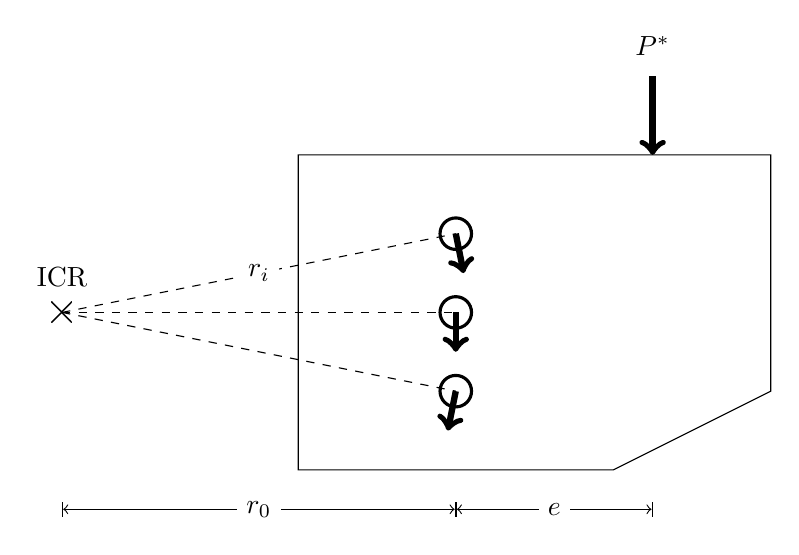
\begin{tikzpicture}
\draw(-1,-1)--++(4,0)--++(2,1)--++(0,3)-|cycle;
\foreach\x in{1}{
\foreach\y in{0,1,2}{
\draw(\x,\y)node[circle,inner sep=0pt,minimum size=4mm,line width=.4mm,draw]{};}}
\draw[->,line width=.8mm](3.5,4)node[above=1mm]{$P^*$}--++(0,-1);
\draw[|<->|](1,-1.5)--(3.5,-1.5)node[midway,fill=white]{$e$};
\draw[|<->|](-4,-1.5)--(1,-1.5)node[midway,fill=white]{$r_0$};
\draw[dashed](-4,1)node{\LARGE\texttimes}node[above=2mm]{ICR}--(1,1);
\draw[dashed](-4,1)--(1,2)node[midway,fill=white]{$r_i$}(-4,1)--(1,0);
\draw[->,line width=.8mm](1,2)--++(.1,-.5);
\draw[->,line width=.8mm](1,1)--++(0,-.5);
\draw[->,line width=.8mm](1,0)--++(-.1,-.5);
\end{tikzpicture}\caption{Illustration of ICR}
\end{figure}

According to this method, the deformation of each fastener (or part of a weld) is assumed to be proportional to its distance from the ICR. The connection fails when on of the fasteners reaches the maximum deformation $\Delta_{max}$. Accordingly, the maximum resistance is denoted as $R_{ult}$.

It is also necessary to know the force deformation relationship for each bolt. A linear relationship can be expressed as
\begin{gather}\label{eq:ri_linear}
R_i=R_{ult}\dfrac{\Delta_i}{\Delta_{max}},
\end{gather}
where $R_{ult}$ is the ultimate dependable resistance of a bolt in shear.

This relationship does not have to be linear. For example, according to AISC tables, the deformation relationship is given by the following exponential equation.
\begin{gather}\label{eq:ri}
R_i=R_{ult}\left(1-e^{-0.394\Delta_i}\right)^{0.55}.
\end{gather}
\begin{figure}[H]
\centering\footnotesize
\begin{tikzpicture}
\begin{axis}[
width=10cm,height=7cm,
axis x line=middle,
axis y line=middle,
xlabel=$\Delta_i$,
ylabel=$R_i$,
ytick=\empty,
xtick=\empty,
xmin=-1,
ymin=-.1,
xmax=12,
ymax=1.2,
]
\addplot[domain=0:8.6,samples=100,line width=.8mm]{(1-exp(-.394*x))^.55}node[midway,above=2mm,rotate=15]{exponential \eqsref{eq:ri}};
\addplot[dashed,domain=0:8.6,samples=2,line width=.8mm]{(1/8.6*x}node[midway,below=2mm,rotate=38]{linear \eqsref{eq:ri_linear}};
\draw[cc0066,dashed](axis cs:8.6,.981)node{\LARGE\texttimes}--(axis cs:8.6,0)node[below]{$\Delta_{max}=\SI{8.6}{\mm}$};
\end{axis}
\end{tikzpicture}\caption{Linear and nonlinear responses}
\end{figure}

The procedure is iterative.
\begin{itemize}
\item Assume location of ICR ($r_0$)
\item Check equilibrium\\For vertical $P$ only, there are
\begin{align}
\sum{}F_x=0,\quad&\longrightarrow\quad\sum{}R_i\dfrac{y_i}{r_i}=0,\quad\text{Since there is only vertical applied load.}\\
\sum{}F_y=0,\quad&\longrightarrow\quad\sum{}R_i\dfrac{x_i}{r_i}=P_{u1},\\
\sum{}M=0,\quad&\longrightarrow\quad\sum{}R_i\dfrac{r_i}{e+r_0}=P_{u2},
\end{align}
where $R_i=R_i\left(\Delta_i\right)$ is \eqsref{eq:ri} (or \eqsref{eq:ri_linear}) and $\Delta_i=\dfrac{r_i}{r_{max}}\Delta_{max}$, in which
\begin{conditions}
r_i&distance from ICR to bolt $i$\\
r_{max}&distance to the farthest bolt
\end{conditions}
This assumes the farthest bolt(s) would reach the maximum deformation $\Delta_{max}$.
\item Iterate on $r_0$ until $P_{u1}=P_{u2}$\\Such iteration can be tedious so tables are often made for standard connections.
\end{itemize}

For friction--grip (slip critical) connections, the force $R_i$ may be assumed to be constant for all fasteners. It is the dependable friction resistance per bolt.
\begin{exmp}
Ultimate Strength Method on Bolt Group

Use ultimate strength method to analyse the previous example.
\end{exmp}
\begin{solution}
From the previous example, the demand causes the maximum shear force \SI{76}{\kn} while the capacity per bolt is \SI{92.6}{\kn}, thus the maximum $P^*$ is
\begin{gather*}
P^*=\SI{120}{\kn}\times\dfrac{\SI{92.6}{\kn}}{\SI{76}{\kn}}=\SI{146.2}{\kn}.
\end{gather*}

Knowing $\Delta_{max}=\SI{8.6}{\mm}$, $e=\SI{300}{\mm}$ and $R_{ult}=\SI{92.6}{\kn}$.

Try $r_0=\SI{39.33}{\mm}$, using \textbf{linear} relationship \eqsref{eq:ri_linear},
\begin{table}[H]
\centering
\begin{tabular}{cccccccccc}
	\toprule
	         & \multicolumn{2}{c}{About c.r.} & \multicolumn{2}{c}{About ICR} &          &            &          &          &          \\
	Bolt No. &  $x_i$   &        $y_i$        &  $x_i$   &       $y_i$        &   $r$    & $\Delta_i$ &  $R_i$   & $P_{u1}$ & $P_{u2}$ \\
	         & \si{\mm} &      \si{\mm}       & \si{\mm} &      \si{\mm}      & \si{\mm} &  \si{\mm}  & \si{\kn} & \si{\kn} & \si{\kn} \\ \midrule
	   1     &   -80    &         -90         &  -40.67  &        -90         &  98.76   &    5.68    &  61.19   &  -25.19  &  17.81   \\
	   2     &   -80    &          0          &  -40.67  &         0          &  40.67   &    2.34    &  25.19   &  -25.19  &   3.02   \\
	   3     &   -80    &         90          &  -40.67  &         90         &  98.76   &    5.68    &  61.19   &  -25.19  &  17.81   \\
	   4     &    80    &         -90         &  119.33  &        -90         &  149.47  &    8.60    &  92.60   &  73.93   &  40.79   \\
	   5     &    80    &          0          &  119.33  &         0          &  119.33  &    6.87    &  73.93   &  73.93   &  26.00   \\
	   6     &    80    &         90          &  119.33  &         90         &  149.47  &    8.60    &  92.60   &  73.93   &  40.79   \\ \bottomrule
	         &          &                     &          &     $r_{max}$      &  149.47  &            &  $\sum$  &  146.21  &  146.21
\end{tabular}
\end{table}
It can be noted that this method is identical to standard elastic method since bolt deformation is linear elastic.

Try $r_0=\SI{62.76}{\mm}$, using \textbf{exponential} relationship \eqsref{eq:ri},
\begin{table}[H]
\centering
\begin{tabular}{cccccccccc}
	\toprule
	         & \multicolumn{2}{c}{About c.r.} & \multicolumn{2}{c}{About ICR} &          &            &          &          &          \\
	Bolt No. &  $x_i$   &        $y_i$        &  $x_i$   &       $y_i$        &   $r$    & $\Delta_i$ &  $R_i$   & $P_{u1}$ & $P_{u2}$ \\
	         & \si{\mm} &      \si{\mm}       & \si{\mm} &      \si{\mm}      & \si{\mm} &  \si{\mm}  & \si{\kn} & \si{\kn} & \si{\kn} \\ \midrule
	   1     &   -80    &         -90         &  -17.24  &        -90         &  91.64   &    4.67    &  84.20   &  -15.84  &  21.27   \\
	   2     &   -80    &          0          &  -17.24  &         0          &  17.24   &    0.88    &  47.11   &  -47.11  &   2.24   \\
	   3     &   -80    &         90          &  -17.24  &         90         &  91.64   &    4.67    &  84.20   &  -15.84  &  21.27   \\
	   4     &    80    &         -90         &  142.76  &        -90         &  168.76  &    8.60    &  90.87   &  76.87   &  42.27   \\
	   5     &    80    &          0          &  142.76  &         0          &  142.76  &    7.27    &  89.66   &  89.66   &  35.29   \\
	   6     &    80    &         90          &  142.76  &         90         &  168.76  &    8.60    &  90.87   &  76.87   &  42.27   \\ \bottomrule
	         &          &                     &          &     $r_{max}$      &  168.76  &            &  $\sum$  &  164.61  &  164.61
\end{tabular}
\end{table}

For exponential relationship, $P_u=\SI{164.61}{\kn}$ corresponds to $\SI{12}{\percent}$ increase in strength due to nonlinearity. Inelastic ICR method can be used for welds too.
\end{solution}
\section{Eccentric Bolted Tension Shear Connections}
These connections have complex behaviour and several methods have been proposed for design as described by \citet{Smith1996}. We consider proof loaded high strength bolts here and we will use the method \citep{Salmon2009} where high strength bolt forces are used to prevent lift-off.
\begin{figure}[H]
\centering\footnotesize
\begin{tikzpicture}[scale=.8,ext/.pic={
\path[fill=white](-0.2,0)to[bend left](0,0.1)to[bend right](0.2,0.2)to(0.2,0)to[bend left](0,-0.1)to[bend right](-0.2,-0.2)--cycle;
\draw(-0.2,0)to[bend left](0,0.1)to[bend right](0.2,0.2) (0.2,0)to[bend left](0,-0.1)to[bend right](-0.2,-0.2);
}]
\draw(0,0)--++(3,0)--++(2,1)--++(0,2)-|cycle;
\draw(0,.2)--++(3.4,0)(0,2.8)--++(5,0)(.2,.2)--++(0,2.6);
\draw(0,3.8)rectangle++(-2,-4.5);
\draw(-.2,3.8)--++(0,-4.5)(-1.8,3.8)--++(0,-4.5);
\draw(-1,3.8)pic[rotate=90]{ext}++(0,-4.5)pic[rotate=90]{ext};
\foreach\x in{.325,.975,1.625,2.275}{
\draw[fill=black](-.2,.1+\x)rectangle(.2,.3+\x);
\draw[dashed,cc0066,line width=.4mm](-.4,.2+\x)--++(.8,0);
\foreach\y in{6.45,7.55}
\node[draw,circle,inner sep=0,minimum size=2.5mm,line width=.4mm]at(\y,.2+\x){};
}
\draw[<-,line width=.6mm](3,3)--++(0,1)node[left]{$V^*_u$};
\draw[<-,line width=.6mm](2,1.5)--++(1,0)node[right]{$N^*_u$};
\draw[|<->|](0,3.5)--++(3,0)node[midway,fill=white]{$e$};
\draw(6,0)rectangle++(2,3)(6.9,0)rectangle++(.2,3);
\draw[|<->|](8.3,0)--++(0,.525)node[midway,right=2mm]{$p/2$};
\draw[|<->|](8.3,.525)--++(0,.65)node[midway,right=2mm]{$p$};
\draw[|<->|](8.3,.525+.65)--++(0,.65)node[midway,right=2mm]{$p$};
\draw[|<->|](8.3,.525+.65*2)--++(0,.65)node[midway,right=2mm]{$p$};
\draw[|<->|](8.3,.525+.65*3)--(8.3,3)node[midway,right=2mm]{$p/2$};
\draw[|<->|](5.7,0)--++(0,3)node[midway,fill=white]{$d$};
\draw[|<->|](6,3.4)--++(2,0)node[midway,fill=white]{$b$};
\draw[dashed](11,-.5)node[below,align=center]{stress\\due to $N^*_u$}--++(0,4);
\draw[draw,fill=black!10](11,0)rectangle++(-1,3);
\draw[dashed](13,-.5)node[below,align=center]{stress\\due to $V^*_ue$}--++(0,4);
\draw[draw,fill=black!10](13,0)--++(0,3)--++(1,0)--++(-2,-3)--cycle;
\draw[dashed](16,-.5)node[below,align=center]{total stress}--++(0,4);
\draw[draw,fill=black!10](16,0)--++(0,3)--++(.5,0)--++(-2.5,-3)--cycle;
\node at(12,1.5){\Large$+$};
\node at(14.5,1.5){\Large$=$};
\end{tikzpicture}\caption{Stress components of eccentrically loaded bolted connection}
\end{figure}
The compressive stress due to $N^*=\sum{}N^*_{tf}$ can be computed as
\begin{gather}
f_{bolt}=\dfrac{\sum{}N^*_{tf}}{bd}.
\end{gather}
The tensile stress on the \textbf{top} bolt due to $M^*=V_u^*e$ can be computed as
\begin{gather}
f_{plate}=\dfrac{M^*}{I}y=\dfrac{V_u^*e}{bd^3/12}\left(\dfrac{d}{2}-\dfrac{p}{2}\right)=6V_u^*e\dfrac{d-p}{bd^3}.
\end{gather}
Bolt forces only increase significantly after the applied stress becomes greater than $f_{bolt}$ and lift-off occurs. The limit is
\begin{gather*}
f_{bolt}\geqslant{}f_{plate}\qquad\longrightarrow\qquad
\dfrac{\sum{}N^*_{tf}}{bd}\geqslant{}6V_u^*e\dfrac{d-p}{bd^3}.
\end{gather*}
Thus,
\begin{gather}
M^*=V_u^*e\leqslant\dfrac{\sum{}N^*_{tf}}{bd}\dfrac{1}{6}\dfrac{bd^3}{d-p},\quad\longrightarrow\quad
M^*=V_u^*e\leqslant\dfrac{\sum{}N^*_{tf}}{6}\dfrac{d^2}{d-p}.
\end{gather}
Noting that due to the presence of shear force $V_u^*$, $N^*_{tf}$ shall be reduced by considering combined action (see \S~\ref{sec:bolt_combined} and \S~\ref{sec:bolt_combined_s}).
\clearpage
\begin{exmp}
Find $P^*$ considering M20X/8.8/S bolts. Two 125\texttimes75\texttimes12UA angles are used in the connection with short leg connected to beam and long leg connected to plate. A vertical force $P^*$ is applied on bolt line connecting plate (\SI{75}{\mm} from column surface).
\begin{figure}[H]
\includegraphics[height=6cm]{PIC/CH08/BTC}\hfill
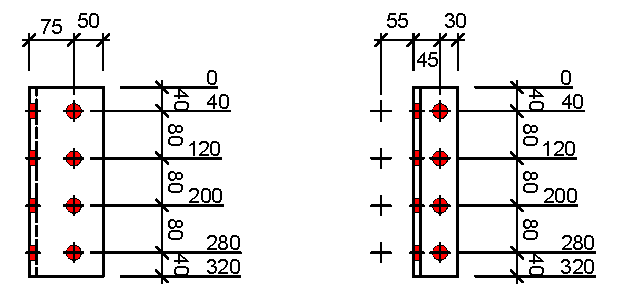
\includegraphics[height=5cm]{PIC/CH08/BTCD}
\end{figure}
\end{exmp}
\begin{solution}
\begin{align*}
M^*=P^*e&\leqslant\dfrac{\sum{}N^*_{tf}}{6}\dfrac{d^2}{d-p},\\
P^*&\leqslant\dfrac{1}{\SI{75}{\mm}}\times\dfrac{8N^*_{tf}}{6}\times\dfrac{\SI{320}{\mm}\times\SI{320}{\mm}}{\SI{320}{\mm}-\SI{80}{\mm}}=7.59N^*_{tf}.
\end{align*}
Or, $N^*_{tf}\geqslant0.132P^*$.
\begin{gather*}
V^*_f=\dfrac{P^*}{n}=0.125P^*.
\end{gather*}
For M20X/8.8/S bolts,
\begin{gather*}
\phi{}N_{tf}=\SI{163}{\kn},\qquad
\phi{}V_f=\SI{129}{\kn}.
\end{gather*}
Consider combined action,
\begin{align*}
\left(\dfrac{V^*_{f}}{\phi{}V_{f}}\right)^2+\left(\dfrac{N^*_{tf}}{\phi{}N_{tf}}\right)^2&\leqslant1.0,\\
\left(\dfrac{0.125P^*}{\SI{129}{\kn}}\right)^2+\left(\dfrac{0.132P^*}{\SI{163}{\kn}}\right)^2&\leqslant1.0,\\
P^*&\leqslant\SI{792.3}{\kn}.
\end{align*}
Using a friction--type connection (/TB), assume $k_h=1.0$, consider combined action,
\begin{align*}
\dfrac{V^*_{f}}{\phi{}V_{f}}+\dfrac{N^*_{tf}}{\phi{}N_{tf}}&\leqslant1.0,\\
\dfrac{0.125P^*}{\SI{35.5}{\kn}}+\dfrac{0.132P^*}{\SI{101.5}{\kn}}&\leqslant1.0,\\
P^*&\leqslant\SI{207.5}{\kn}.
\end{align*}
\end{solution}
\section{Welded Eccentric Shear Connections}
\subsection{Elastic Method}
It is assumed that the connector plate is rigid, the welds do not deform, the forces result from direct shear and torsion. Rotation is assumed to occur about the weld centroid.
\begin{figure}[H]\centering\footnotesize
\begin{tikzpicture}[scale=1.2,ext/.pic={
\path[fill=white](-0.2,0)to[bend left](0,0.1)to[bend right](0.2,0.2)to(0.2,0)to[bend left](0,-0.1)to[bend right](-0.2,-0.2)--cycle;
\draw(-0.2,0)to[bend left](0,0.1)to[bend right](0.2,0.2) (0.2,0)to[bend left](0,-0.1)to[bend right](-0.2,-0.2);
}]
\draw[dashed](.5,-2)--++(0,4);
\draw(1.5,-1.5)rectangle(-.5,1.5);
\draw[fill=white](0,-1)rectangle(3,1);
\draw[dashed](.3,-2)--++(0,4)node[midway,circle,fill=black,inner sep=0,minimum size=2mm]{}node[midway,below right=2mm,align=center]{centriod\\of weld};
\draw(.5,-1.5)pic[rotate=90]{ext}++(0,3)pic[rotate=90]{ext};
\draw[line width=1.2mm](1.5,-1)-|(0,1)--++(1.5,0);
\draw[<-,line width=.6mm](2.5,1)--++(0,1.2)node[left]{$P^*_u$};
\draw[|<->|](.3,1.8)--(2.5,1.8)node[midway,fill=white]{$e$};
\begin{scope}[xshift=5cm]
\draw[dashed](.3,-1.5)--++(0,3)node[midway,circle,fill=black,inner sep=0,minimum size=2mm]{};
\draw[line width=1.2mm](1.5,-1)-|(0,1)--++(1.5,0);
\setstructmech{convention=direction,node=cc0066,linewidth=.6mm}
\NodalForce{.3,0}[N][-P^*_u][-P^*_ue][1.5]
\draw[line width=1.2mm,cc0066](1.5,1)--++(-.2,0);
\draw[dashed](.3,0)--(1.4,1)coordinate(A);
\draw[-stealth,line width=.6mm,00cc66](A)--++(1/1.5,-1.1/1.5)coordinate(B)node[midway,right=2mm,align=left]{torsion\\component};
\draw[-stealth,line width=.6mm,0066cc](B)--++(0,-.8)coordinate(C)node[midway,right=2mm,align=left]{shear\\component};
\draw[-stealth,line width=.6mm](A)--(C)node[midway,left=2mm,align=left]{total\\stress};
\end{scope}
\end{tikzpicture}
\caption{Stress components of weld element}
\end{figure}
\begin{figure}[ht!]
\centering
\includegraphics[width=.9\textwidth]{PIC/CH08/SW}
\caption{Treating welds as lines \citep{Roark2012}}\label{fig:weld_line}
\end{figure}
\subsubsection{Analysis Procedure}
\begin{itemize}
\item Determine centroid of weld
\begin{gather*}
\bar{x}=\dfrac{\displaystyle\int{}x\md{A}}{\displaystyle\int\md{A}}=\dfrac{\displaystyle\sum{}Ax}{\displaystyle\sum{}A},\qquad
\bar{y}=\dfrac{\displaystyle\int{}y\md{A}}{\displaystyle\int\md{A}}=\dfrac{\displaystyle\sum{}Ay}{\displaystyle\sum{}A}.
\end{gather*}
\item Calculate polar moment of inertia $J$
\begin{gather*}
J=\int{}r^2\md{A}=\int{}\left(x_i^2+y_i^2\right)\md{A}=\int{}x_i^2\md{A}+\int{}y_i^2\md{A}=I_x+I_y,
\end{gather*}
where
\begin{conditions}
x_i=x-\bar{x}&$x$ distance measured from centroid\\
y_i=y-\bar{y}&$y$ distance measured from centroid
\end{conditions}
By parallel axis theorem,
\begin{gather*}
J=\sum{}I_{x0}+\sum{}I_{y0}+\sum{}Ax_i^2+\sum{}Ay_i^2,
\end{gather*}
where $I_{x0}$ and $I_{y0}$ are moment of inertia about the element's own axes.
\item Calculate components of stress due to direct shear
\begin{gather*}
f'_x=\dfrac{P^*_{u,x}}{A}=\dfrac{P^*_{u,x}}{t_el_w},\qquad
f'_y=\dfrac{P^*_{u,y}}{A}=\dfrac{P^*_{u,y}}{t_el_w}.
\end{gather*}
\item Calculate components of stress due to torsion
\begin{gather*}
f''_x=P^*_ue\dfrac{y_i}{J},\qquad
f''_y=P^*_ue\dfrac{x_i}{J}.
\end{gather*}
\item Calculate components of stress due to any potential out-of-plane moment $M^*$
\begin{gather*}
f_z=M^*\dfrac{y_i}{I_x}+M^*\dfrac{x_i}{I_y}.
\end{gather*}
\item Calculate total stress
\begin{gather*}
f_{u}^*=\sqrt{\left(f'_x+f''_x\right)^2+\left(f'_y+f''_y\right)^2+f_z^2}.
\end{gather*}
\item Find critical point(s) on the weld and ensure
\begin{gather*}
f_{u,max}^*\leqslant\left\{\begin{array}{ll}
\phi_{weld}0.6f_{weld}&\text{weld strength}\\[3mm]
\phi_{steel}0.85\dfrac{t_p}{t_t}0.6f_u&\text{plate block tearing}
\end{array}\right.
\end{gather*}
\end{itemize}
\subsubsection{Design Procedure}
\begin{itemize}
\item Select weld process, strength and weld lines
\item Analyse the connection to find the required throat thickness $t_t$ to resist $P^*$
\item Calculate the weld leg size $t_w$
\item Check shear and tension stresses in the base metal
\end{itemize}
\begin{exmp}\href{run:./WORKSHEET/CH08/EX8.ECLW.sm}{Worksheet} Eccentrically Loaded Weld

A bracket is to be connected to both flanges of a 250UC89.5 Grade 300 column to transit a vertical factored force of \SI{200}{\kn} that is \SI{200}{\mm} from the column. Assume plate satisfies all necessary requirements. Use E48XX GP electrodes and find weld size.
\begin{figure}[H]\footnotesize
\begin{tikzpicture}[scale=1,ext/.pic={
\path[fill=exmpbg](-0.2,0)to[bend left](0,0.1)to[bend right](0.2,0.2)to(0.2,0)to[bend left](0,-0.1)to[bend right](-0.2,-0.2)--cycle;
\draw(-0.2,0)to[bend left](0,0.1)to[bend right](0.2,0.2) (0.2,0)to[bend left](0,-0.1)to[bend right](-0.2,-0.2);
}]
\draw[dashed](.5,-2.5)--++(0,5);
\draw(1.5,-2)rectangle(-.5,2);
\draw[fill=exmpbg](0,-1)rectangle(4,1);
\draw(.5,-2)pic[rotate=90]{ext}++(0,4)pic[rotate=90]{ext};
\draw[line width=1.2mm](1.5,-1)-|(0,1)--++(1.5,0);
\draw[<-,line width=.6mm](3.5,1)--++(0,1.2)node[left]{$P^*_u$};
\draw[|<->|](1.5,1.8)--(3.5,1.8)node[midway,fill=exmpbg]{$\SI{200}{\mm}$};
\draw[|<->|](0,-2.5)--++(1.5,0)node[midway,fill=exmpbg]{$\SI{150}{\mm}$};
\draw[|<->|](-1,-1)--++(0,2)node[midway,fill=exmpbg,rotate=90]{$\SI{200}{\mm}$};
\draw[<-](2,-.8)--++(1,-.8)--++(2,0)node[fill=exmpbg]{\SI{12}{\mm} plate};
\begin{scope}[xshift=6.5cm]
\draw[dashed](.45,-1.5)--++(0,3)node[midway,circle,fill=black,inner sep=0,minimum size=2mm]{};
\draw[line width=1.2mm](1.5,-1)-|(0,1)--++(1.5,0);
\draw[|<->|](0,-1.5)--++(.45,0)node[midway,below]{$\bar{x}$};
\draw[|<->|](0,-2)--++(1.5,0)node[midway,fill=exmpbg]{$\SI{150}{\mm}$};
\draw[|<->|](-1,-1)--++(0,2)node[midway,fill=exmpbg,rotate=90]{$\SI{200}{\mm}$};
\end{scope}
\node at(11,0){\includegraphics[height=5cm]{PIC/CH08/WJ}};
\end{tikzpicture}
\end{figure}
\end{exmp}
\begin{solution}
Welds are subject to shear and torsion.

Since there are two sides, each side experiences $\SI{200}{\kn}/2=\SI{100}{\kn}$ force.
\begin{itemize}
\item Determine centroid of weld
\begin{gather*}
\bar{x}=\dfrac{\displaystyle\sum{}Ax}{\displaystyle\sum{}A}=\dfrac{2\times\SI{150}{\mm}\times\dfrac{\SI{150}{\mm}}{2}}{\SI{200}{\mm}+2\times\SI{150}{\mm}}=\SI{45}{\mm}.
\end{gather*}
\item Calculate polar moment of inertia $J$, ignoring any high order terms of $t_t$,
\begin{align*}
J&=2\times\underbrace{\SI{150}{\mm}\times{}t_t\times\left(\SI{100}{\mm}\right)^2}_\text{$Ay_i^2$ of horizontal elements}
+\underbrace{\dfrac{t_t\times\left(\SI{200}{\mm}\right)^3}{12}}_\text{$I_x$ of vertical element}\\
&+2\times\underbrace{\dfrac{t_t\times\left(\SI{150}{\mm}\right)^3}{12}}_\text{$I_y$ of horizontal elements}
+2\times\underbrace{\SI{150}{\mm}\times{}t_t\times\left(\SI{75}{\mm}-\SI{45}{\mm}\right)^2}_\text{$Ax_i^2$ of horizontal elements}\\
&+\underbrace{\SI{200}{\mm}\times{}t_t\times\left(\SI{45}{\mm}\right)^2}_\text{$Ax_i^2$ of vertical element}\\
&=\dfrac{14712500}{3}t_t\approx4904166.7t_t.
\end{align*}
The factor $4904166.7$ can alternatively be computed via the formula provided in \figref{fig:weld_line}.
\item Calculate components of stress due to direct shear
\begin{gather*}
f'_y=\dfrac{P_{u,y}}{A}=\dfrac{\SI{200}{\kn}/2}{500t_t}=\dfrac{0.2}{t_t}.
\end{gather*}
\item Calculate components of stress due to torsion\\
The critical points are top and bottom right ends.
\begin{gather*}
f''_x=P_ue\dfrac{y_{i,max}}{J}=\SI{200}{\kn}/2\times\left(\SI{200}{\mm}+\SI{105}{\mm}\right)\times\dfrac{\SI{100}{\mm}}{4904166.7t_t}=\dfrac{0.622}{t_t},\\
f''_y=P_ue\dfrac{x_{i,max}}{J}=\SI{200}{\kn}/2\times\left(\SI{200}{\mm}+\SI{105}{\mm}\right)\times\dfrac{\SI{105}{\mm}}{4904166.7t_t}=\dfrac{0.653}{t_t}.
\end{gather*}
\item Calculate total stress
\begin{align*}
f_{u}^*&=\sqrt{\left(f''_x\right)^2+\left(f'_y+f''_y\right)^2}\\
&=\sqrt{\left(\dfrac{0.622}{t_t}\right)^2+\left(\dfrac{0.2}{t_t}+\dfrac{0.653}{t_t}\right)^2}\\
&=\dfrac{\SI{1.056}{\kn\per\mm}}{t_t}.
\end{align*}
\item Check capacity
\begin{gather*}
\dfrac{\SI{1.056}{\kn\per\mm}}{t_t}\leqslant\phi_{weld}0.6f_{weld},\quad\longrightarrow\quad
t_t\geqslant\dfrac{\SI{1.056}{\kn\per\mm}}{0.6\times0.6\times\SI{480}{\mpa}}=\SI{6.11}{\mm}.
\end{gather*}
\item Check block tearing in plate
\begin{align*}
\dfrac{\SI{1.056}{\kn\per\mm}}{t_t}&\leqslant\phi_{steel}0.85\dfrac{t_p}{t_t}0.6f_u\\
\dfrac{\SI{1.056}{\kn\per\mm}}{t_t}&\leqslant0.9\times0.85\times\dfrac{\SI{12}{\mm}}{t_t}\times0.6\times\SI{440}{\mpa}=\dfrac{\SI{2.424}{\kn\per\mm}}{t_t}.
\end{align*}
\end{itemize}
Thus required weld size is $t_w=\sqrt{2}\times\SI{6.11}{\mm}=\SI{8.64}{\mm}$, try \SI{10}{\mm} weld. The minimum size is \SI{5}{\mm}. The maximum size is \SI{11}{\mm}. Use \SI{10}{\mm} E48XX GP fillet welds.
\end{solution}
\begin{exmp}
Compute required size of W50X fillet weld. Assume that column and bracket do no govern. Assume the shear stress is uniform.
\begin{figure}[H]
\footnotesize
\begin{tikzpicture}[scale=1,ext/.pic={
\path[fill=exmpbg](-0.2,0)to[bend left](0,0.1)to[bend right](0.2,0.2)to(0.2,0)to[bend left](0,-0.1)to[bend right](-0.2,-0.2)--cycle;
\draw(-0.2,0)to[bend left](0,0.1)to[bend right](0.2,0.2) (0.2,0)to[bend left](0,-0.1)to[bend right](-0.2,-0.2);
}]
\draw(0,0)--++(3,0)--++(2,1)--++(0,2)-|cycle;
\draw(0,3.8)rectangle++(-2,-4.5);
\draw(-.2,3.8)--++(0,-4.5)(-1.8,3.8)--++(0,-4.5);
\draw(-1,3.8)pic[rotate=90]{ext}++(0,-4.5)pic[rotate=90]{ext};
\draw[<-,line width=.6mm](3,3)--++(0,1)node[left]{\SI{65}{\kn}};
\draw[|<->|](0,3.5)--++(3,0)node[midway,fill=exmpbg]{\SI{150}{\mm}};
\draw[|<->|](-2.5,0)--++(0,3)node[midway,fill=exmpbg,rotate=90]{\SI{250}{\mm}};
\draw[line width=1.2mm](0.06,0)--++(0,3);
\draw(0,.5)--++(2,-1)--++(1,0)--++(-.3,.3)--++(0,-.6)node[left=1mm]{$t_w$}node[right=1mm]{250}--++(.3,.3)--++(1,0)coordinate(A)node[right=2mm]{W50X GP};
\draw(A)--++(.2,.2)(A)--++(.2,-.2);
\draw[<-](2,.8)--++(1,.8)--++(2,0)node[fill=exmpbg]{\SI{12}{\mm} plate};
\begin{scope}[xshift=7cm]
\draw[line width=1.2mm](-.2,0)--++(0,3);
\draw[line width=1.2mm](.2,0)--++(0,3);
\draw[dashed,->](-.5,1.5)--(.5,1.5)node[right]{$x$};
\draw[dashed,->](0,-.5)--++(0,4)node[right]{$y$};
\draw[dashed](1.5,-.5)node[below]{shear stress}--++(0,4);
\draw[draw,fill=black!10](1.5,0)rectangle++(1,3);
\draw[dashed](4,-.5)node[below]{bending stress}--++(0,4);
\draw[draw,fill=black!10](4,0)--++(0,3)--++(1,0)--++(-2,-3)--cycle;
\end{scope}
\end{tikzpicture}
\end{figure}
\end{exmp}
\begin{solution}
Compute stress due to shear force, assume shear stress is uniformly distributed.
\begin{gather*}
f'_y=\dfrac{N^*}{A}=\dfrac{\SI{65}{\kn}}{2\times250\times{}t_t}=\dfrac{\SI{0.13}{\kn\per\mm}}{t_t}.
\end{gather*}
Compute stress due to moment.
\begin{gather*}
I_x=2\times\dfrac{t_t\times\left(\SI{250}{\mm}\right)^3}{12}=2604166.7t_t.
\end{gather*}
Thus,
\begin{gather*}
f_{z,max}=M^*\dfrac{y_{max}}{I_x}=\SI{65}{\kn}\times\SI{150}{\mm}\times\dfrac{\SI{125}{\mm}}{2604166.7t_t}=\dfrac{\SI{0.468}{\kn\per\mm}}{t_t}.
\end{gather*}
The total stress is then
\begin{gather*}
f_u^*=\sqrt{\left(\dfrac{\SI{0.13}{\kn\per\mm}}{t_t}\right)^2+\left(\dfrac{\SI{0.468}{\kn\per\mm}}{t_t}\right)^2}=\dfrac{\SI{0.486}{\kn\per\mm}}{t_t}.
\end{gather*}
Check capacity.
\begin{gather*}
\dfrac{\SI{0.486}{\kn\per\mm}}{t_t}\leqslant\phi_{weld}0.6f_{weld},\quad\longrightarrow\quad
t_t\geqslant\dfrac{\SI{0.486}{\kn\per\mm}}{0.6\times0.6\times\SI{480}{\mpa}}=\SI{2.81}{\mm}.
\end{gather*}
Thus, $t_w=\sqrt{2}\times\SI{2.81}{\mm}=\SI{3.98}{\mm}$. The minimum size is \SI{5}{\mm}. Use \SI{5}{\mm} W50X GP fillet welds.
\end{solution}
